\subsection{Empiryczna złożoność czasowa parsowania}
Biorąc pod uwagę szeroki zakres wydajności na Rysunku 11, można by posądzać o nieliniowe
zachowanie dla wolniejszych parserów. Aby prześledzić, wykreślimy czas parsowania według
wielkości pliku na Rysunku 13 i narysujemy regresję najmniejszych kwadratów
i krzywej dopasowania danych LOWESS [6].
\begin{figure}[h]
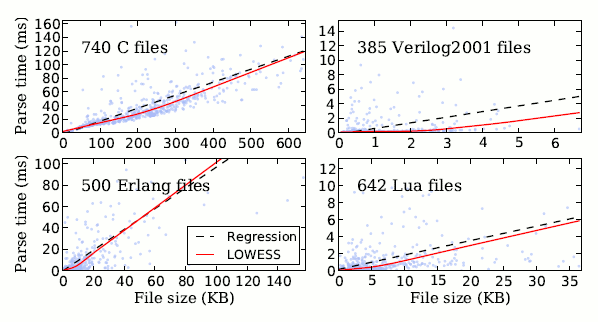
\includegraphics[scale=0.67]{Figure13.png}
\caption{
Liniowy czas pasowania vs wielkość pliku. Regresja liniowa (linia przeywana)
i nieskrępowana krzywa LOWESS zbiegają się dając silny dowód liniowości
Krzywe obliczone na (dolne) 99\% weilkości plików ale powiększone
aby pokazać szczegóły dolnego 40\% czasu parsowania.
}
\end{figure}
Krzywe LOWESS są parametrycznie nieskrępowane (nie wymagane aby były linią lub
jakimś szczególnym wielomianem) i one wirtualnie odzwierciedlają każdą
linię regresji, dostarczając silnego dowodu że relacja
pomiędzy czasem parsowania a wielkością wejścia jest liniowa.
Ta sama metodologia pokazuje że parser wygenerowany z gramatyki nie-SLL (nie pokazane)
wzięty ze specyfikacji C11 jest również liniowy, pomimo że dużo wolniejszy niż nasza wersja SLL.
\par
Powinniśmy jeszcze zobaczyć nieliniowe zachowanie w praktyce ale teoretyczne
zachowanie najgorszego przypadku parsowania ALL(*) jest O($n^4$). Eksperymentalne
dane czasu parsowania dla następującej wymyślonej gramatyki najgorszego przypadku
wykazuje zachowanie czwartego stopnia dla wejścia a, aa, aaa,
..., $a^n$ (z n $\leqslant$ 120 symboli mogliśmy przetestować w rozsądnym czasie).
//
S $\rightarrow$ A, A $\rightarrow$ aAAj|aA|a.
//
Generowany parser wymaga predykcji na każdym symbolu wejściowym
i każda predykcja musi badać cały pozostały input.
Operacja closure wykonana dla każdego symbolu unput musi badać
całą głębokość GSS, która może być rozmiaru n, Ostatecznie, łączenie
dwóch GSS może zająć O(n) w naszej implementacji, dając
złożoność O($n^4$).
\par
Z naszych eksperymentów otrzymaliśmy że przeniesienie analizy gramatyki
do czasu parsowania do dania ALL(*) siły jest nie tylko praktyczne
ale daje ekstremalnie wydajne parsery, rywalizujące z
ręcznie dostrajanymi rekurencyjnymi parserami kompilatora Javy.
Pamiętanie rezultatów analizy w DFA jest krytyczne do takiej wydajności.
Mimo teoretycznej złożoności O($n^4$), w praktyce ALL(*) zdaje się by liniowe
i nie wykazuje nieprzewidzianego zachowania jeśli chodzi o czas lub
pamięć jak ogólne algorytmy.

